\chapter{Results and Conclusions}

The injection locking was successful and we successfully produced two working beams with an adjustable detuning. 

\section{Spectrum Analyzer}
In this section, we discuss the spectrum analyzer that we built to analyze this system. 

\begin{figure}
%    \centerline{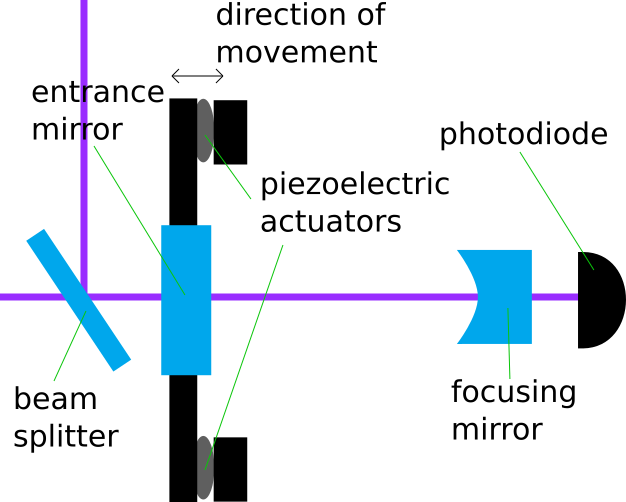
\includegraphics[trim=100pt 100pt 100pt 100pt, clip=true, totalheight=0.5\textheight,angle=90]{spectrumAnalyzer}}
    \centerline{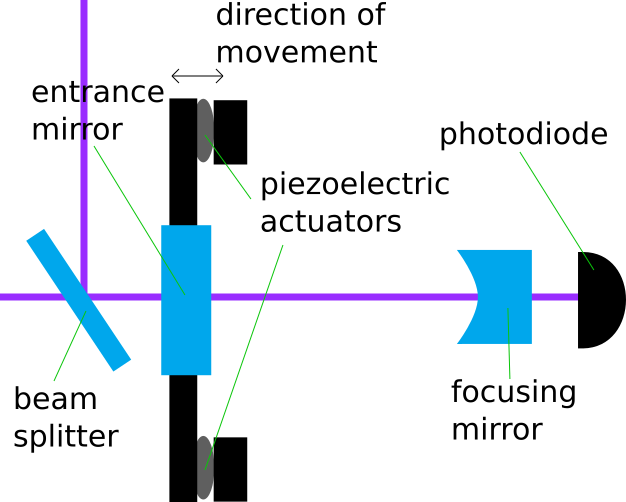
\includegraphics[totalheight=0.3\textheight ]{spectrumAnalyzer}}
    %\includegraphics[totalheight=0.3\textheight]{testfigure}
    \caption[]{\label{fig:spectrumAnalyzer}
    A diagram of the spectrum analyzer. both lasers are coupled to the cavity. One of the mirrors is mounted on piezoelectric devices that allow fine control of its motion. 
}
\end{figure}

The spectrum analyzer is a semiconfocal cavity of length 200 mm. The flat, partially reflective mirror through which light enters the cavity is mounted on a mount that features piezo-electric actuators. At the other end is a curved mirror of focal length 200 mm. Behind this is a photodiode \footnote{the Thorlabs DET XXXXX--probably a DET100A/M or something similar.}.

This is accomplished using a commercially available sweeping piezo control box. 

The length of the optical cavity in the spectrum analyzer can be modulated by sweeping the voltage that we put across the piezoelectric crystals. When the cavity length is such that the coupled light is close to a resonance of the cavity, we expect to see higher signal on the photodiode. 

In order to calculate the Free Spectral Range (FSR) of the cavity, we search for the amount by which the frequency of the coupled light must change as we move from one resonance to the other. 

According to Ref.\ \cite{lasersMilonniEberly}, the equation for the resonant frequencies of the longitudinal modes of our cavity are

\begin{equation} \label{eqModeF}
\nu_{qmn}=\frac{c}{2L}\left[q + \frac{1}{\pi}(m+n+1)\cos^{-1}(\operatorname{sgn}(g_1)\sqrt{g_1 g_2})\right], 
\end{equation}

if we model the resonant modes as Laguerre-Gaussian modes. Here, $L$ is the length of the cavity; $q$ is a nonnegative integer; $m$ and $n$ are integers representing the order of the Hermite polynomials in the solution in the $x$ and $y$ directions. $g_i$ is defined for each mirror and is given by $1-L/R_i$.


From the equation, we see that the hemiconfocal cavity has the special property that many of the resonances align. One of our mirrors is flat, so $g_1=1-L/\infty=1$, while the other's focal length, $f_2$ is equal to the length of the cavity. Recalling that the normal relationship between radius of curvature and focal length is $R_2=2 f_2$, we see that $g_2=1-L/R_2=1-L/(2 f_2)=1-L/(2 L)=1/2$. Thus, 

\begin{equation}
\cos^{-1}(\operatorname{sgn}(g_1)\sqrt{g_1 g_2})=\frac{\pi}{4}.
\end{equation}
Substituting this into Eq.\ \ref{eqModeF}, we see that 

\begin{equation}\label{freq_semiconfocal}
\nu_{qmn}=\frac{c}{2L}\left[q + \frac{1}{4}(m+n+1)\right], 
\end{equation}

Since $m$,$n$ and $q$ are all integers, we see that the resonant modes will be integer multiples of $c/(8L)$. Eq.\ \ref{freq_semiconfocal} also demonstrates one of the nicest features about semi-confocal cavities, which is that different transverse modes of the electric and magnetic have the same resonant frequency. Thus, rather than having to couple carefully to the TEM$_{00}$ mode, we can allow the light to couple to any transverse mode of the cavity. If we assume that we are coupled to many cavity modes, we can safely assume that adjacent resonant frequency peaks are separated by $c/8L$, which is the Free Spectral Range of the cavity. 

Interestingly, the hemiconfocal configuration has an advantage over \footnote{I am going out on a limb here...} the confocal configuration that is illustrated by this equation. In the confocal configuration, both mirrors are identical and are placed so that their focal points coincide. This means that $L=R_1/2=R_2/2$ and thus $g_1=1-L/R_1=g_2=1-L/(2L-R_2)$. Therefore, $\sqrt{g_1g_2}=0$, making the free spectral range of the cavity $c/4L$. However, note that if $L$ changes, then the sign of $g_1$ changes, leading to a kink in the frequency response. With a hemiconfocal cavity, there is no such discontinuity. This makes the expansion in the next section slightly easier. 

Note that we are note actually scanning the frequency of the laser. Rather, it is the length of the cavity that scans. Note, however, that both confocal and hemiconfocal cavities remain good, stable cavities as their lengths are scanned since the condition for cavity stability is that $0\leq g_1 g_2 \leq 1$. 

The piezoelectric mount (Thorlabs KC1-PZ) is rated to accept a maximum voltage of 150 V and provide a maximum of $\pm4\mu$m of linear travel. Thus, since our sweep voltage is only about 75 V, we expect that our cavity should be sweeping ~2$\mu$m. If the wavelength of the light is 408 nm, we expect that for each 2$\mu$m of displacement, we should see about $8*2\mu$m$/408nm \approx 40$ resonant peaks. This is a good order of magnitude estimate for the most peaks we can see. Therefore, we can say that the change in cavity length, $\Delta L< 2\mu$m.

Now, if we take Eq.\ \ref{eqModeF} and make the following substitutions:
\begin{align}
g_1&\rightarrow1 \text{ (since $R_1=\infty$)} \\
g_2&\rightarrow 1-L/(2L)\\
L&\rightarrow L(1-\epsilon)\\
\end{align},

we get 

\begin{equation} \label{eqModeF_ready_for_expansion}
\nu_{qmn}=\frac{c}{2L(1+\epsilon)}\left(q+\frac{m+n+1}{\pi}\arccos(\sqrt{1-L(1-\epsilon)/(2L)})\right)
\end{equation}.

Note that we have used $R_2=2L$ and not $R_2=2L(1+\epsilon)$ since the radius of the mirror does not change as we sweep the cavity. 

We now make a Taylor expansion of Eq.\ \ref{eqModeF_ready_for_expansion} using Mathematica, we get 
\begin{align*}
\nu_{qmn}=\frac{c}{8L}\biggl((4q+m+n+1) +\\
 \left(-4q-m-n-1+\frac{2}{\pi}(1+m+n)\right)\epsilon+\\
 \left(4q+m+n+1+\frac{2}{\pi}(1+m+n))\right)\epsilon^2\\
 \left(-4q-m-n-1+\frac{7}{3\pi}(1+m+n)\right)\epsilon^3\\
 \left(4q+m+n+1-\frac{7}{3\pi}(1+m+n)\right)\epsilon^4\\
\biggr)
\end{align*}

The coefficient for the first order expansion in terms of $\epsilon$ contains integers $m$,$n$ and $q$ as we expect. 
However, it might seem unnerving at first that it also contains coefficents like $2/\pi$ that are of order unity! The reason this is ok is that $q>>m,n$. We know this is the case for two reasons: First, the Laguerre Gaussian modes are derived using the paraxial wave approximation. The paraxial wave equation assumes solutions of the form
\begin{equation}
\vec{E}(\vec{r},t)=E(\vec{r})\exp[i(kz-\omega t)]
\end{equation}
and it relies on the fact that 
\begin{equation}
\left|2k\frac{\partial E(\vec{r})}{\partial z}\right|\gg\left|\frac{\partial^2E(\vec{r})}{\partial z^2}\right|
\end{equation}
Since the derivatives of $E(\vec{r})$ depend on $m$th and $n$th order Hermite polynomials, we see that our equations only hold up when $m$ and $n$ are reasonably small. 

This can also be easily seen since the cavity length is 20cm, while the cavity mirrors are scarcely 1 cm across and the laser modes in the cavity can be seen to be less than 5 mm in diameter. One may imagine intuitively that the number of nodes along a long dimension (represented roughly by $q$) is going to be large compared to the number of nodes created by light at the same frequency along a much smaller distance. 

\footnote{Now, I'm not sure whether it's the case that our approximation breaks down and that's why the $m$ and $n$ have to be small. It seems intuitive to me that you can get a lot more oscillations at a given frequency in a 20cm space than you can in a 1 cm space, but I'm not sure if that's the right intuition.\cite{lasersMilonniEberly} eq. 7.8.17 might have some decent insight. All the modes have the same $R(z)$ and $w(z)$, but I think there's more power out of the bucket as they say.  }

This might be OK. If, for example, we assume the argument in the radical ($1-L(1+\epsilon)/(2L)\approx 1/2$ for all values of $\epsilon$, then we get this expansion: 

\begin{align}
\nu_{qmn}=\frac{c}{8L}
\end{align}



If we assume that we are coupled to many different modes, we can assume that the nearest peaks on our spectrum analyzer represent a change of 

It would, of course, be possible, to suppress some of the modes by coupling our beam in carefully, 

A simple ray-tracing argument can also be used. 
\begin{figure}
\centerline{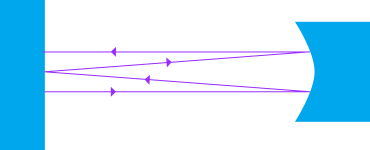
\includegraphics[height=3cm]{spectrum_analyzer_path.png}}
\caption{Illustration of the optical path that makes a complete trip around the semiconfocal cavity. Note that the ray traverses the entire length of the path four times before doubling back on itself. It traverses the path 8 times before ending up in the same place again. This diagram similar to one found on page 277 of Ref.\ \cite{lasersMilonniEberly}}
\end{figure}

In order for the cavity to be resonant with our light, the full optical path of the light must be an integer number of wavelengths. The resonance condition is 
\begin{equation}
n \lambda = d
\end{equation}
where $n$ is an integer, $\lambda$ is the wavelength and $n$ is the length of the optical path in the cavity. 
For a semiconfocal cavity, we see that a ray parallel to the optical axis would have to traverse the cavity length 8 times before finally getting back to its starting point. 

This argument may prove that any mode of the cavity will find resonances spaced by $c/8L$.

%Probably there is some way in which we can talk about a Gaussian mode that makes the Gouy phase shift somehow explainable in terms of two (or more!) crossing rays of propagation. 



Perhaps the resonant length of the other modes is not because they travel farther off-axis. It's perhaps related to some other issue that arises when we move the focal points.




First, we examine the output of the spectrum analyzer when we couple both Slave lasers into it. 
The two peaks clearly correspond to the two slave lasers. We can see that there is a lot of power \footnote{honestly, I'm not sure that all the power coming out was in those modes. It was a little bit flaky}
We can clearly identify which peak corresponds to which Slave laser by blocking one of the slaves. 

\section{}

Next, we attempt an experiment whereby we adjust the driving frequency. We should be able to see the peaks shifting by an amount corresponding to the change in the frequency. This will provide strong evidence that the two slaves are, in fact, injection locked to the modulated beams coming out of the AOM. 

This test has the further benefit of confirming that we have calculated the free spectral range of the cavity in the spectrum analyzer correctly. 

%where is the energy going? I think it goes from reflecting to transmitting

 
\begin{figure}
    %\centerline{\includegraphics[trim=100pt 100pt 100pt 100pt, clip=true, totalheight=0.5\textheight,angle=90]{testfigure}}
    %\centerline{\includegraphics[totalheight=0.3\textheight]{testfigure}}
    \centerline{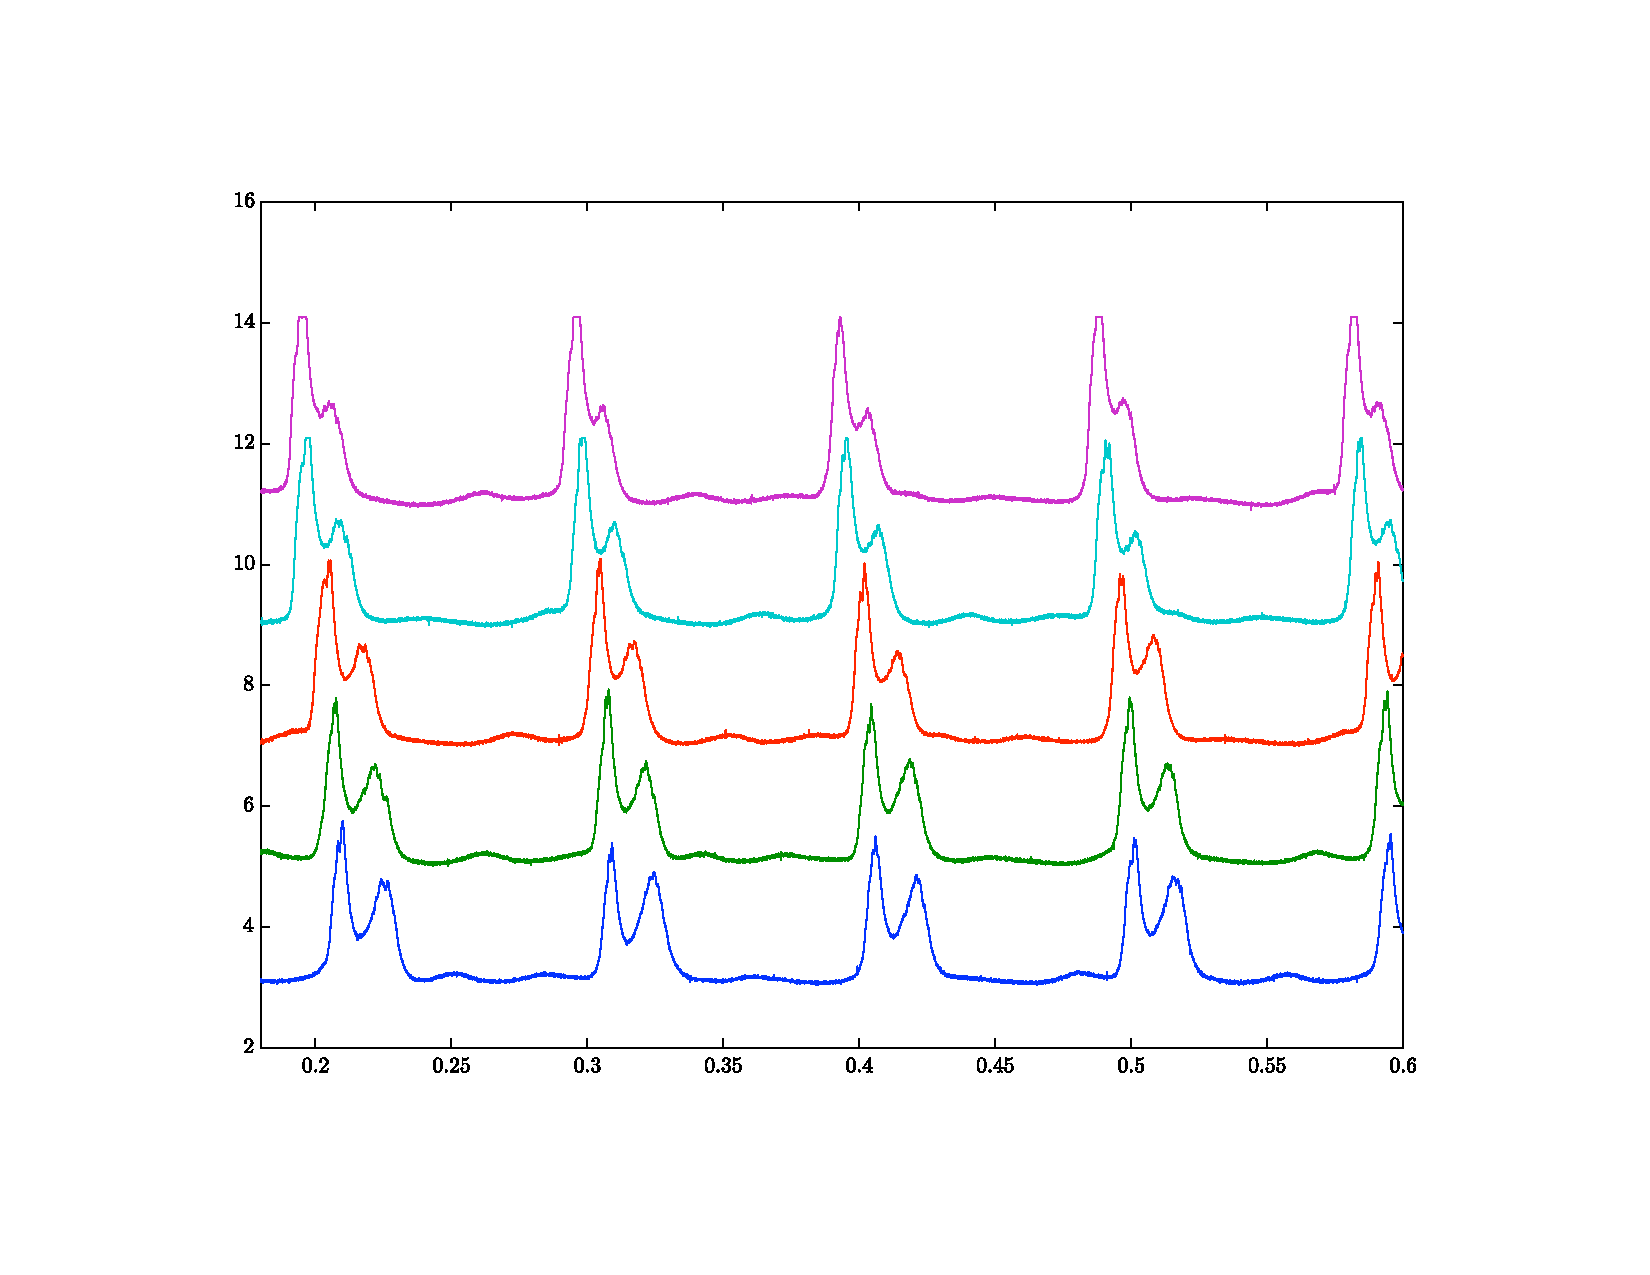
\includegraphics{sampleOffsetData}}
    %\includegraphics[totalheight=0.3\textheight]{testfigure}
    \caption[]{\label{fig:typicaldata}
    We changed the detuning on our frequency generator in something like 10 MHz increments. These are some of the data that we have that show the spacing between our peaks changing in a predictable way.}
\end{figure}
\begin{figure}
\centerline{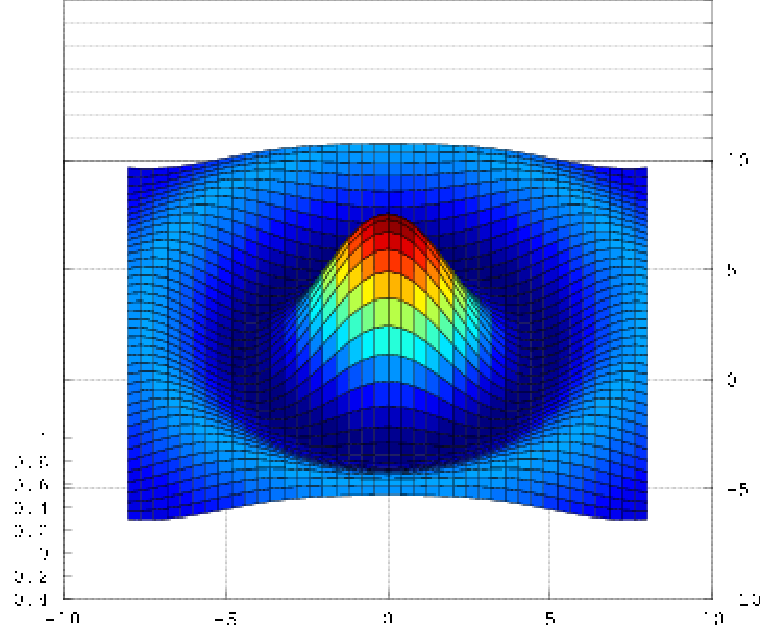
\includegraphics{thisone}}
\end{figure}

\begin{figure}
\centerline{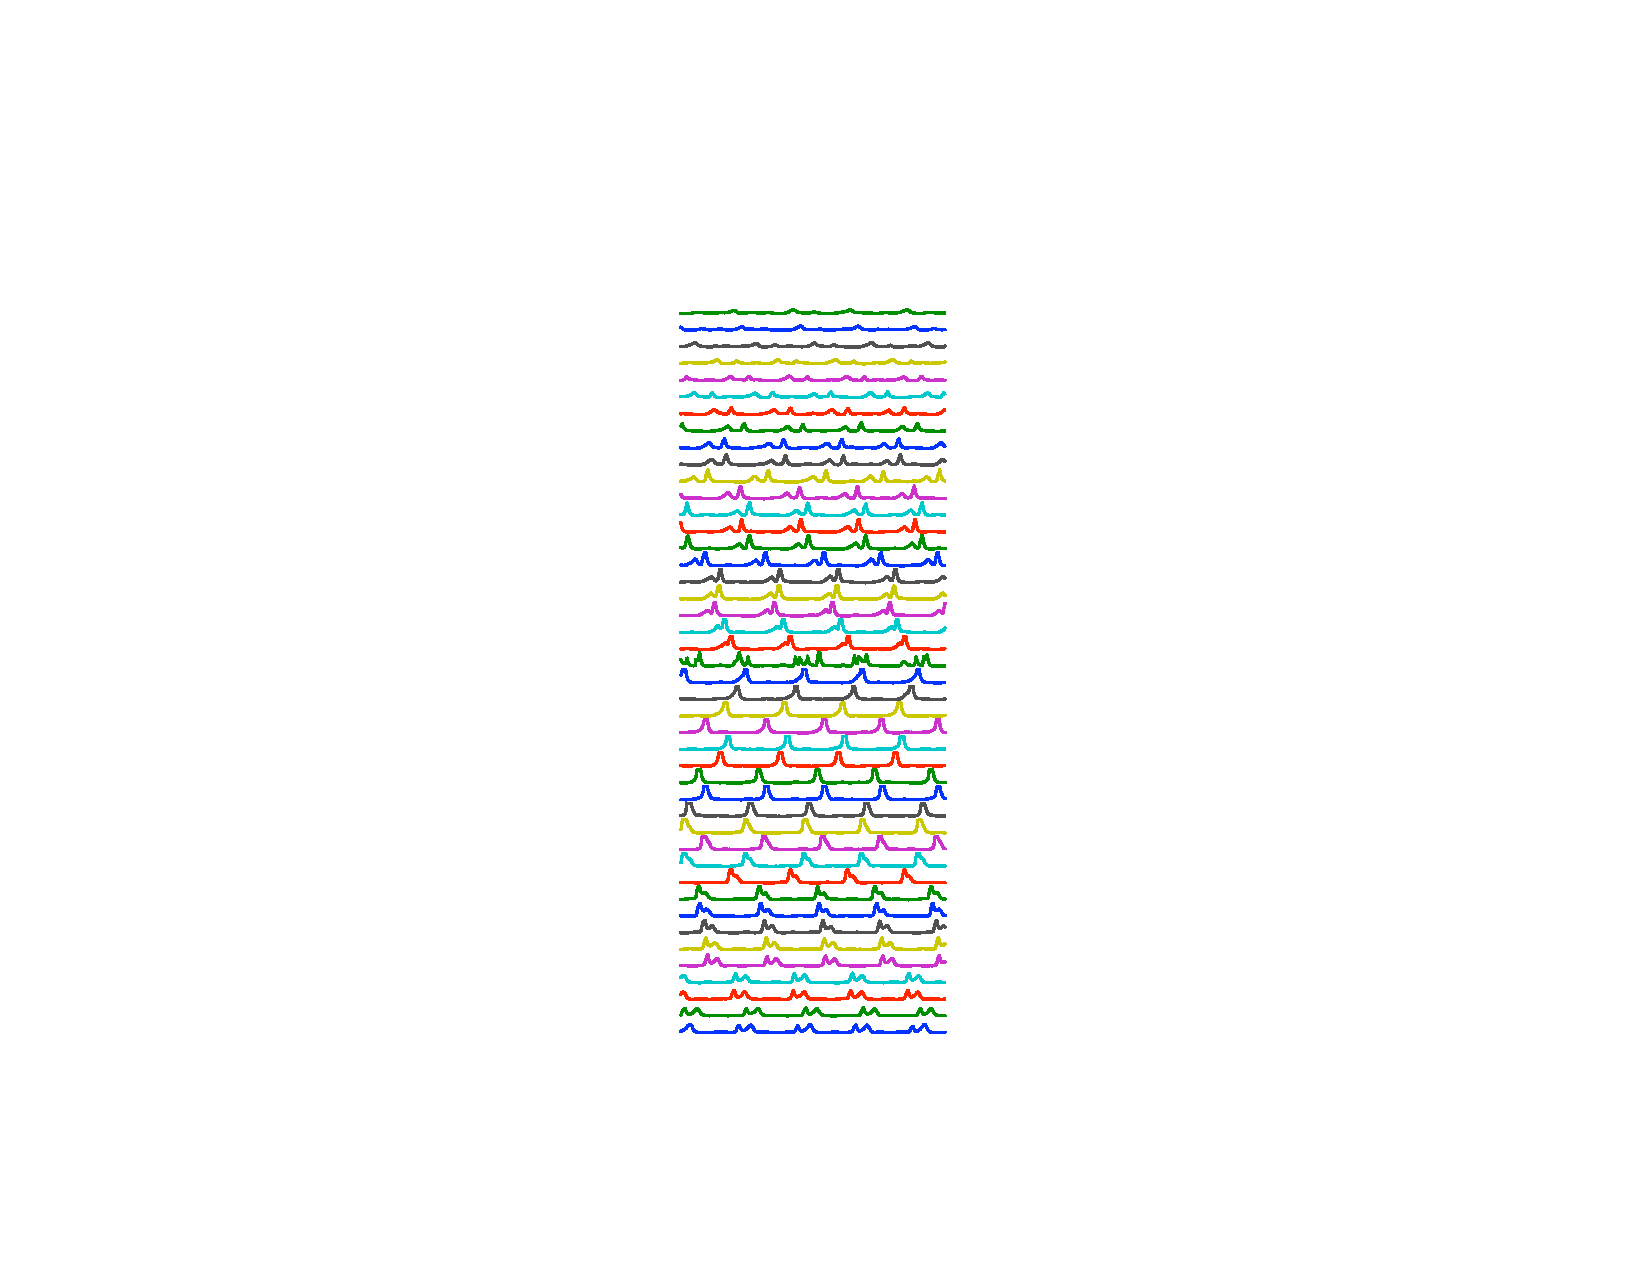
\includegraphics{all_splittingData}}
\caption[]{\label{fig:alldata} 
This is the complete set of data from which the previous graphic was culled. Some of it is clipped uglily. The peaks are on top of each other, but it may have drifted to a higher power between when I set it up and when I took the data. I'm not sure why this looks so much worse than the data I normally take.}
\end{figure}

Also, I have data that I can analyze to examine the feasibility of a Chu lock. I recorded 999 traces that showed the output of the spectrum analyzer, the current and the voltage. I recorded these over several hours, during which the laser drifted into and out of good, single mode operation. In principle, this data could be analyzed. 

We have shown that we can change the oscillator frequency and thereby change the detuning. There is a limit to the extent that we can do this. (Notice in Fig.\ \ref{fig:alldata} that the peaks get small as we continue to detune.) However, this is due to geometry. When I realigned using the method of measuring the photocurrent coming out of the slave lasers, I found that I was able to get the thing to work over an entirely different range of oscillator frequencies. 

